\mySection{5.1 Introduction}
%-------------- start slide -------------------------------%{{{ 5.4
\begin{frame}
   % {\S\: 5.1 Introduction}

 {\bf\noindent Motivating example}: Given an unfair coin, or $p$-coin, such that
 \[
 X=
 \begin{cases}
    1 & \text{head with probability $p$},\\
    0 & \text{tail with probability $1-p$,}
 \end{cases}
 \]
 how would you determine the value $p$?
 \vfill
{\bf Solutions:~}
 \begin{enumerate}
  \item You need to try the coin several times, say, three times. What you obtain is ``HHT''.
  \item Draw a conclusion from the experiment you just made.
 \end{enumerate}

 \end{frame}


 \begin{frame}[fragile]

 {\bf\noindent Rationale:~} The choice of the parameter $p$ should be the value that maximizes the probability of the sample.
 \vfill
 \begin{align*}
 \PP(X_1=1,X_2=1,X_3=0) = &
 P(X_1=1)P(X_2=1)P(X_3=0) \\
 = &p^2(1-p).
 \end{align*}
 \vfill
 \pause
\begin{minipage}{0.4\textwidth}
\begin{lstlisting}
# Hello, R.
p <- seq(0,1,0.01)
plot(p,p^2*(1-p),
     type="l",
     col="red")
title("Likelihood")
# add a vertical dotted (4) blue line
abline(v=0.67, col="blue", lty=4)
# add some text
text(0.67,0.01, "2/3")
 \end{lstlisting}
\end{minipage}
\hfill
\begin{minipage}{0.5\textwidth}
 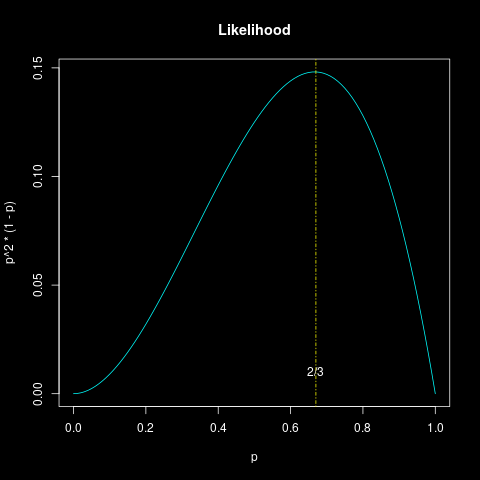
\includegraphics[scale=0.25]{Bernoulli-neg.png}
\end{minipage}
\vfill
Maximize $f(p) = p^2(1-p)$ ....
\end{frame}
%-------------- end slide -------------------------------%}}}
%-------------- start slide -------------------------------%{{{ 5.5
\begin{frame}[fragile]

{\bf A random sample of size $n$ from the population -- Bernoulli$(p)$}: \\[1em]
\begin{itemize}
 \item $X_1, \cdots, X_n$ are i.i.d.\footnote{independent and identically distributed} random variables, each following Bernoulli$(p)$. \\[1em]
 \item Suppose the outcomes of the random sample are: $X_1=k_1,\cdots,X_n=k_n$. \\[1em]
 \item What is your choice of $p$ based on the above random sample?
 \vfill
 \item[]
 \[
 p=\frac{1}{n} \sum_{i=1}^n k_i =: \bar{k}.
 \]
\end{itemize}

\end{frame}
%-------------- end slide -------------------------------%}}}
%-------------- start slide -------------------------------%{{{ 5.6
\begin{frame}

{\bf A random sample of size $n$ from the population with given pdf}: \\[1em]

\begin{itemize}
 \item $X_1, \cdots, X_n$ are i.i.d. random variables, each following the same given pdf.
 \vfill
 \item a {\bf statistic} or an {\bf estimator} is a function of the random sample. \\
 \begin{center}
  \alert{Statistic/Estimator is a random variable!}
 \end{center}
 e.g.,
 \[
 \widehat{p} = \frac{1}{n} \sum_{i=1}^n X_i.
 \]
 \vfill
 \item The outcome of a statistic/estimator is called an {\bf estimate}. e.g.,
 \[
 p_e = \frac{1}{n} \sum_{i=1}^n k_i.
 \]
\end{itemize}
\end{frame}
%-------------- end slide -------------------------------%}}}
